\clearpage
\section{Kreuzvorhersage innerer Dynamiken}
\label{sec:exp_inner_prediction}
Bei Messungen der elektrischen Erregung des Herzens können nach aktuellem Stand meist nur die Erregungen auf der Herzoberfläche gemessen werden. Die Ausbreitungen im Inneren des räumlich ausgedehnten Herzens bleiben somit verborgen. Zudem ist anzunehmen, dass die Gesamtdynamik nicht nur durch die Oberfläche, sondern auch durch die Erregung im Inneren bestimmt und charakterisiert wird. Somit kommt die Frage auf, ob die innere Erregung des Herzens ausschließlich durch die Kenntnis der Oberflächendynamik vorhergesagt werden kann. In diesem Abschnitt soll versucht werden, diese Fragestellung erneut mit den \textsc{ESN}s und den klassischen Methoden zu untersuchen. Dabei wird diese Frage statt an einem dreidimensionalen System an den zuvor bereits benutzten zweidimensionalen Modellen untersucht.\\

\begin{figure}[h]
	\centering
	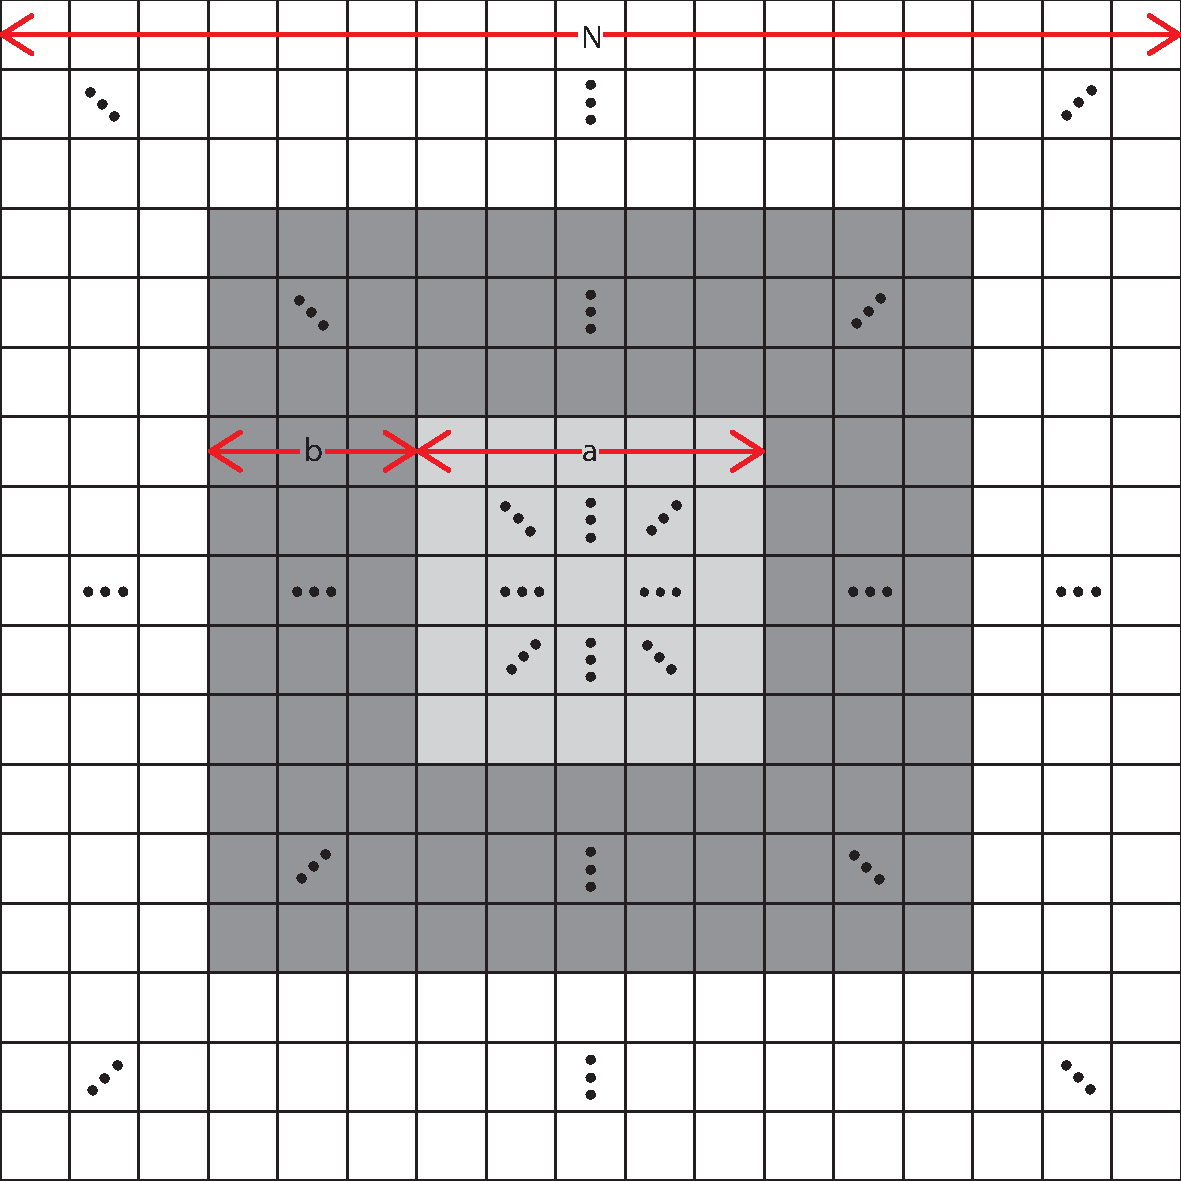
\includegraphics[width=.6\linewidth]{figures/illustrations/inner_prediction.pdf}
	\caption{Darstellung des Aufbaus. Das gesamte $N \times N$ große Feld der Spannungsvariable ist in weiß, wohingegen der vorherzusagende Bereich der Größe $a \times a$ in hellgrau dargestellt ist. Drumherum liegt der dunkelgraue Rahmen der Breite $b$ dessen Pixel für die Vorhersage des Inneren genutzt werden.}
	\label{fig:exp_inner_prediction}
\end{figure}

Hierbei wird nur das Feld der Spannungsvariable betrachtet. In diesem $N \times N$ Einheiten großen Feld wird ein Quadrat mit der Seitenlänge $a$ ausgewählt, für dessen Pixel die Spannungsvariable bestimmt werden soll. Dazu wird um das innere Quadrat ein Rahmen der Breite $b$ gewählt und die Spannungsvariable der beinhalteten Pixel als Quelle genutzt. Eine graphische Illustration dieses Aufbaus ist in Abbildung \ref{fig:exp_inner_prediction} dargestellt. Somit wird die Spannung im Inneren für $a^2$ Punkte durch die Kenntnis der $(a+2b)^2-a^2$ umgebenden Pixel vorhergesagt.\\

Dieses Szenario ist für die in Tabelle \ref{tab:exp_inner_cross_pred_parameter} angegebenen Parameterkombinationen durchgeführt worden. Im Folgenden werden jeweils nur die gefundenen Hyperparameter und Ergebnisse für den $b$-Wert vorgestellt, der zu dem geringsten Fehler führt.

\begin{table}[h]
	\centering
	\begin{tabular}{cccc|ccc|ccc|ccc|ccc|ccc|cc|c}
		\hline
		$a$ & \multicolumn{3}{c|}{4} & \multicolumn{3}{c|}{8} & \multicolumn{3}{c|}{16} & \multicolumn{3}{c|}{32} & \multicolumn{3}{c|}{64} & \multicolumn{3}{c|}{128*} & \multicolumn{2}{c|}{146*} & 148* \\
		\hline
		$b$ & 1 & 2 & 3 & 1 & 2 & 3 & 1 & 2 & 3 & 1 & 2 & 3 & 1 & 2 & 3 & 1 & 2 & 3 & 2 & 1 & 1 \\
		\hline
	\end{tabular} 
	\caption{Verwendete Parameter $a$ und $b$ für die Abmessungen des inneren und äußeren Quadrates. Die mit * markierten Werte sind nur für die \textsc{ESN}s untersucht worden.}
	\label{tab:exp_inner_cross_pred_parameter}
\end{table} 

\subsection{Nächste-Nachbar-Vorhersage}
Für die letzte Aufgabe ist zuerst der \textsc{NN}-Ansatz getestet worden. Es ist anzumerken, dass dieser nicht für alle Parameterkombinationen $a$, $b$ aus Tabelle \ref{tab:exp_inner_cross_pred_parameter} durchgeführt worden ist, da der Rechenaufwand teilweise zu groß geworden ist. Dies ist darauf zurückzuführen, dass die Dimension der Eingabevariablen mit
\begin{align*}
(a+2b)^2-a^2 = 4b^2+4ab
\end{align*}
skaliert. Diese Dimensionalität wird mit der Dimension der Verzögerungskoordinaten noch vervielfacht, wie bereits in Kapitel \ref{sec:experiments_general_classical} beschrieben. Da zudem die Rechenzeit für diesen Ansatz nach \ref{sc:theory_nn} für wachsende Dimensionen sehr stark zunimmt, kann diese Aufgabe für große Abmessungen des vorherzusagendenen Bereiches nicht mehr in einer angebrachten Zeit berechnet werden.
Die optimalen gefundenen Hyperparameter und die damit erreichten Ergebnisse sind in Tabelle \ref{tab:exp_inner_cross_nn_results} aufgelistet.

\begin{table}[h]
	\centering

	\begin{tabular}{ccccccccccc}
		\hline		
		\multicolumn{1}{c}{} & \multicolumn{5}{c}{Barkley}\\ 
		\hline 
		\rule[-1ex]{0pt}{2.5ex} $a$ & 4 & 8 & 16 & 32 & 64\\ 
		\rule[-1ex]{0pt}{2.5ex} $b$ & 1 & 1 & 1  & 1  & 1 \\ 
		\rule[-1ex]{0pt}{2.5ex} $\delta$ & 3 & 3 & 4 & 3 & 3 \\ 
		\rule[-1ex]{0pt}{2.5ex} k & 5 & 5 & 5 & 4 & 5 \\ 
		\rule[-1ex]{0pt}{2.5ex} Laufzeit [s] & $\approx 1$ & 8 & 287 & 1809 & 14754\\ 
		\rule[-1ex]{0pt}{2.5ex} \textbf{MSE} & \textbf{0.00368} & \textbf{0.01572} & \textbf{0.09410} & \textbf{0.20458} & \textbf{0.26571}\\ 
		\rule[-1ex]{0pt}{2.5ex} \textbf{NRMSE} & \textbf{0.3517} & \textbf{0.3914} & \textbf{0.7726} & \textbf{1.1640} & \textbf{1.2963} \\ 
		\hline 
	\end{tabular} 
	
	\vspace{0.75cm}

	\centering

	\begin{tabular}{ccccccccccc}
		\hline
		\multicolumn{1}{c}{} & \multicolumn{5}{c}{Mitchell-Schaeffer} \\ 
		\hline 
		\rule[-1ex]{0pt}{2.5ex} $a$ & 4 & 8 & 16 & 32 & 64 \\ 
		\rule[-1ex]{0pt}{2.5ex} $b$ & 1 & 1 & 1  & 1  & 1\\ 
		\rule[-1ex]{0pt}{2.5ex} $\delta$ & 3 & 3 & 3 & 4 & 4 \\ 
		\rule[-1ex]{0pt}{2.5ex} k & 5 & 5 & 5 & 5 & 5 \\ 
		\rule[-1ex]{0pt}{2.5ex} Laufzeit [s] & $\approx 1$ & 17 & 194 & 2482 & 20272\\ 
		\rule[-1ex]{0pt}{2.5ex} \textbf{MSE} & \textbf{0.00463} & \textbf{0.02182} & \textbf{0.08295} & \textbf{0.10699} & \textbf{0.12297} \\ 
		\rule[-1ex]{0pt}{2.5ex} \textbf{NRMSE} & \textbf{0.5160} & \textbf{0.6365} & \textbf{0.9888} & \textbf{1.1646} & \textbf{1.1837} \\ 
		\hline 
	\end{tabular} 

	\caption{Ermittelte Hyperparameter der \textit{Nächsten-Nachbar}-Vorhersage und Werte für $b$ für das \textit{Barkley}-Modell (oben) und das \textit{Mitchell-Schaeffer}-Modell (unten) für verschiedene Größen $a$ des vorherzusagenden Bereichs, welche zu den geringsten Fehlern führen.}
\label{tab:exp_inner_cross_nn_results}
\end{table}

Auffällig ist, dass die Qualität der Vorhersage mit steigendem $a$ stark abnimmt. So kann für das \textit{Barkley}-Modell nur für $a \in \{4,8\}$ ein NRMSE, der deutlich unter $0.50$ liegt, erreicht werden. Für größere Bereiche steigt der NRMSE sogar auf $> 1.0$ an, sodass die Vorhersage nicht mehr präzisere Ergebnisse liefert als eine naive Vorhersage mittels des Mittelwertes des Trainingsdatensatzes. Die Vorhersagen des \textit{Mitchell-Schaeffer}-Modells zeigen eine gleichartige Tendenz, dennoch ist hier der Fehler für die kleinste innere Abmessung $a=4$ deutlich stärker als im \textit{Barkley}-Modell.

\FloatBarrier
\subsection{Radiale Basisfunktionen}
Analog zu den vorherigen Ausführungen sind die radialen Basisfunktionen ebenfalls auf dieses Problem angewendet worden. Dabei ist mit einer analogen Begründung, wie bei den nächsten Nachbarn, nur der eingeschränkte Wertebereich für $a$ durchlaufen worden. Die dafür gefundenen Hyperparameter und die Fehler können der Tabelle \ref{tab:exp_inner_cross_rbf_results} entnommen werden.
\begin{table}[h]
	\centering

	\begin{tabular}{ccccccccccc}
		\hline
		\multicolumn{1}{c}{} & \multicolumn{5}{c}{Barkley}\\ 
		\hline
		\rule[-1ex]{0pt}{2.5ex} $a$ & 4 & 8 & 16 & 32 & 64\\ 
		\rule[-1ex]{0pt}{2.5ex} $b$ & 1 & 1 & 1  & 1  & 1 \\ 
		\rule[-1ex]{0pt}{2.5ex} $\delta$ & 3 & 3 & 4 & 4 & 3 \\ 
		\rule[-1ex]{0pt}{2.5ex} $\sigma_{RBF}$ & 9 & 5 & 9 & 9 & 7\\ 
		\rule[-1ex]{0pt}{2.5ex} Laufzeit [s] & $\approx 1$ & 8 & 45 & 260 & 1839\\ 
		\rule[-1ex]{0pt}{2.5ex} \textbf{MSE} & \textbf{0.00051} & \textbf{0.00450} & \textbf{0.04009} & \textbf{0.08783} & \textbf{0.13903}\\ 
		\rule[-1ex]{0pt}{2.5ex} \textbf{NRMSE} & \textbf{0.0601} & \textbf{0.1909} & \textbf{0.4885} & \textbf{0.8816} & \textbf{0.9805} \\ 
		\hline 
	\end{tabular} 
	
	\vspace{0.75cm}

	\centering

	\begin{tabular}{ccccccccccc}
		\hline
		\multicolumn{1}{c}{} & \multicolumn{5}{c}{Mitchell-Schaeffer} \\ 
		\hline 
		\rule[-1ex]{0pt}{2.5ex} $a$ & 4 & 8 & 16 & 32 & 64 \\ 
		\rule[-1ex]{0pt}{2.5ex} $b$ & 1 & 1 & 1  & 1  & 1\\ 
		\rule[-1ex]{0pt}{2.5ex} $\delta$ & 3 & 3 & 3 & 4 & 4 \\ 
		\rule[-1ex]{0pt}{2.5ex} $\sigma_{RBF}$ & 9 & 9 & 9 & 5 & 7 \\ 
		\rule[-1ex]{0pt}{2.5ex} Laufzeit [s] & $\approx 1$ & 7 & 43 & 237 & 1756\\
		\rule[-1ex]{0pt}{2.5ex} \textbf{MSE} & \textbf{0.00064} & \textbf{0.00497} & \textbf{0.02220} & \textbf{0.04745} & \textbf{0.05588} \\ 
		\rule[-1ex]{0pt}{2.5ex} \textbf{NRMSE} & \textbf{0.0925} & \textbf{0.2842} & \textbf{0.7178} & \textbf{0.9530} & \textbf{1.0094} \\ 
		\hline 
	\end{tabular} 

	\caption{Ermittelte Hyperparameter der radialen Basisfunktionen und Werte für $b$ für das \textit{Barkley}-Modell (oben) und das \textit{Mitchell-Schaeffer}-Modell (unten) für verschiedene Größen $a$ des vorherzusagenden Bereichs, welche zu den geringsten Fehlern führen.}
\label{tab:exp_inner_cross_rbf_results}
\end{table}

Es ist anzumerken, dass der NRMSE für beide Modelle und alle betrachteten Größen $a$ kleiner als $1.0$ bleibt. Nichtsdestotrotz steigt er ebenfalls mit wachsendem $a$ an, wie auch schon bei den nächsten Nachbarn. Für die größten beiden $a$-Werte ist in beiden Modellen der Fehler allerdings schon so groß, dass die Vorhersage kaum nützliche Informationen liefert.

\subsection{Echo State Network}
Im Gegensatz zu den anderen beiden Methoden wächst die benötigte Rechenzeit bei der Verwendung der \textsc{ESN}s nicht so schnell an. Folglich können hiermit auch deutlich größere innere Felder betrachtet werden. Zur Optimierung des Ansatzes ist erneut das in Abschnitt \ref{sec:exp_general_esn} beschriebene Verfahren durchgeführt worden. Es ist allerdings so modifiziert worden, dass bei der groben Hyperparameterbestimmung des \textsc{ESN} vier Punkte, statt wie zuvor ein Punkt, des inneren Quadrates betrachtet worden sind.\\

Zudem ergibt sich bei dieser Aufgabe ein weiteres Problem, das eine Modifikation erfordert: In den vorherigen Aufgaben ist die Dimension des Eingangssignals in das \textsc{ESN} $N_u < 50$ gewesen. Nun wächst die Dimension des Eingangssignals allerdings sehr stark mit $N_u = 4b(b+a)$ an. Dies würde bei der Konstruktion der Eingangsmatrix $\mathbf{W_{in}}$ nach Abschnitt \ref{sec:esn_structure} dazu führen, dass die inneren Einheiten des Reservoirs zu viele Eingangssignale erhalten und somit unter Umständen schnell zu einer Sättigung des $tanh(\cdot)$ in der zeitlichen Entwicklungsgleichung \ref{eq:esn_stateeq} führt. Um dies zu lösen ist ein neuer Hyperparameter $\eta$ eingeführt worden, der die Anzahl von Eingangssignalen pro innerer Einheit beschreibt und somit die Anzahl der Eingangssignale für jede innere Einheit beschränkt. Dadurch wird die Matrix $\mathbf{W_{in}}$ dünn besetzt und enthält pro Zeile $\eta$ Einträge, die ungleich null sind. Dies wird zusätzlich dadurch motiviert, dass viele Einträge des Eingangssignals aus Bildpunkten mit einem geringen Abstand zueinander stammen, wodurch redundante Informationen eingespeist werden würden. Durch eine dünn besetzte Matrix $\mathbf{W_{in}}$ kann dieser Effekt reduziert werden. Des Weiteren wird versucht eine reichhaltigere innere Dynamik durch diesen Schritt, analog zu der Begründung der Dünnbesetztheit der Matrix $\mathbf{W}$, zu erzeugen.\\

Bei der Untersuchung ist auch ersichtlich geworden, dass der untersuchte Bereich der Regularisierung $\lambda \in [\num{5e-2},\num{5e-6}]$ zu gering ist, da der optimale Wert stets am linken Rand des Intervalls gefunden worden ist. Deswegen ist ergänzend eine Suche auf dem größeren Parameterbereich $\lambda \in [\num{5e-4},\num{5e+4}]$ durchgeführt worden.
In Tabelle \ref{tab:exp_inner_cross_esn_results} sind die Fehler und benötigten Laufzeiten für die besten Reservoirs für die beiden Modelle aufgelistet. Die ermittelten Hyperparameter sind in den Tabellen \ref{tab:apx_inner_cross_esn_results_barkley} und \ref{tab:apx_inner_cross_esn_results_ms} aufgeführt. Es kann erneut der Trend beobachtet werden, dass der Fehler mit steigendem $a$ ebenso zunimmt, und der Fehler im \textit{Mitchell-Schaffer}-Modell für kleine Werte für $a$ größer ist als im \textit{Barkley-Modell}.

\begin{table}[h]
	\centering

	\resizebox{\columnwidth}{!}{%
		\begin{tabular}{cccccccc}
			\hline
			\multicolumn{1}{c}{} & \multicolumn{7}{c}{Barkley}\\ 
			\hline 
			\rule[-1ex]{0pt}{2.5ex} $a$ & 4 & 8 & 16 & 32 & 64 & 128 & 148\\ 
			\rule[-1ex]{0pt}{2.5ex} $b$ & 2 & 2 & 2 & 2 & 1 & 2 & 1 \\ 
			\rule[-1ex]{0pt}{2.5ex} Laufzeit [s] & 5 & 15 & 60 & 170 & 1922 & 3320 & 2970\\
			\rule[-1ex]{0pt}{2.5ex} \textbf{MSE} & \textbf{0.00005} & \textbf{0.00111} & \textbf{0.01447} & \textbf{0.09301} & \textbf{0.13093} & \textbf{0.15106} & \textbf{0.18380}\\ 
			\rule[-1ex]{0pt}{2.5ex} \textbf{NRMSE} & \textbf{0.0121} & \textbf{0.0801} & \textbf{0.3386} & \textbf{0.7398} & \textbf{0.9438} & \textbf{1.0098} & \textbf{1.1049} \\ 
			\hline 
		\end{tabular} 
	}
	
	\vspace{0.75cm}

	\centering

	\resizebox{\columnwidth}{!}{%
		\begin{tabular}{cccccccc}
			\hline
			\multicolumn{1}{c}{} & \multicolumn{7}{c}{Mitchell-Schaeffer}\\ 
			\hline
			\rule[-1ex]{0pt}{2.5ex} $a$ & 4 & 8 & 16 & 32 & 64 & 128 & 148\\ 
			\rule[-1ex]{0pt}{2.5ex} $b$ & 1 & 3 & 2 & 2 & 1 & 2 & 1 \\ 
			\rule[-1ex]{0pt}{2.5ex} Laufzeit [s] & 3 & 9 & 27 & 121 & 548 & 3322 & 3021\\
			\rule[-1ex]{0pt}{2.5ex} \textbf{MSE} & \textbf{0.00023} & \textbf{0.00177} & \textbf{0.02969} & \textbf{0.05061} & \textbf{0.06330} & \textbf{0.06842} & \textbf{0.06761}\\ 
			\rule[-1ex]{0pt}{2.5ex} \textbf{NRMSE} & \textbf{0.0661} & \textbf{0.1704} & \textbf{0.6703} & \textbf{0.8861} & \textbf{0.9775} & \textbf{1.0166} & \textbf{1.0049} \\ 
			\hline 
		\end{tabular} 
	}

	\caption{Auflistung der Fehlerwerte MSE und NRMSE zusammen mit der Laufzeit für das jeweils beste \textsc{ESN}, welches zu den geringsten Fehlern führt, für das \textit{Barkley}-Modell (oben) und das \textit{Mitchell-Schaeffer}-Modell (unten) für verschiedene Größen $a$ des vorherzusagenden Bereichs. Dabei ist der Wert für $b$ ebenfalls optimiert worden.}
\label{tab:exp_inner_cross_esn_results}
\end{table}

Es ist anzunehmen, dass für die Vorhersage eines Punktes der weit von den bekannten Randwerten entfernt liegt, nicht nur sein vorheriger Wert und die aktuellen Randwerte benötigt werden. Vielmehr werden die vergangenen Randwerte einen starken Einfluss nehmen. Dies kann anhand eines Beispiels schnell deutlich gemacht werden: Würde eine ebene Welle durch das Feld propagieren, so können weit entfernte Punkte erst deutlich nachdem die Welle durch die Ränder hindurch gelaufen ist, hiervon beeinflusst werden. Somit benötigt das System eine ausgeprägte Gedächtnisleistung. Bei den \textsc{ESN}s skaliert nach \ref{sc:esn} die Gedächtnisleistung mit der Größe $N$ des Netzwerkes. Es wäre also anzunehmen, dass möglichst große Reservoirs eine optimale Leistung erzielen können. Dies kann experimentell nicht bestätigt werden. So erzielen zwar teilweise die größtmöglichen Reservoirs ($N=400$) die besten Ergebnisse, doch gibt es auch Werte für $a$, bei denen kleinere Reservoirs ($N=50$) besser arbeiten.\\

\begin{figure}[H]
	\centering
	\begin{subfigure}{.5\textwidth}
		\centering
		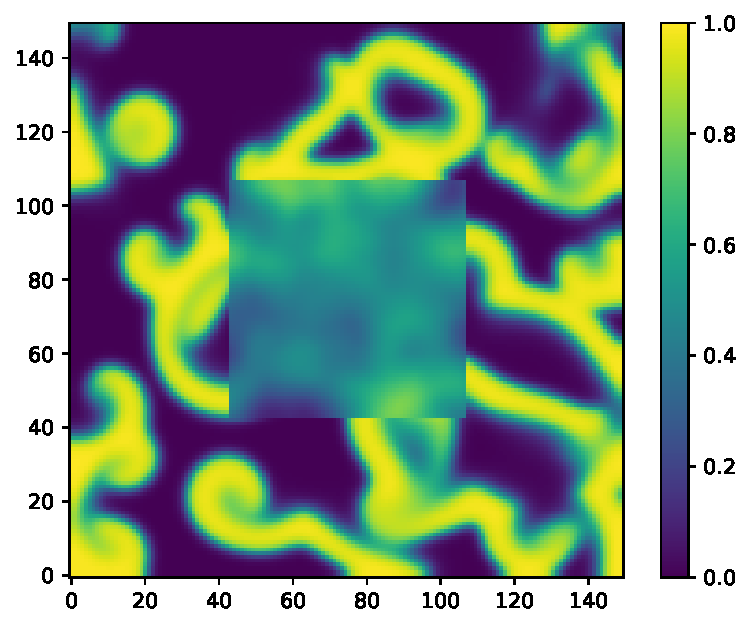
\includegraphics[height=2.5in]{figures/results/inner_cross_prediction/barkley_u_inner_esn_high_penalty.pdf}
		\setcapmargin[1cm]{0.5cm}
		\caption{Vorhersage des \textsc{ESN}s mit $\lambda=50000$}
	\end{subfigure}%
	\begin{subfigure}{.5\textwidth}
		\centering
		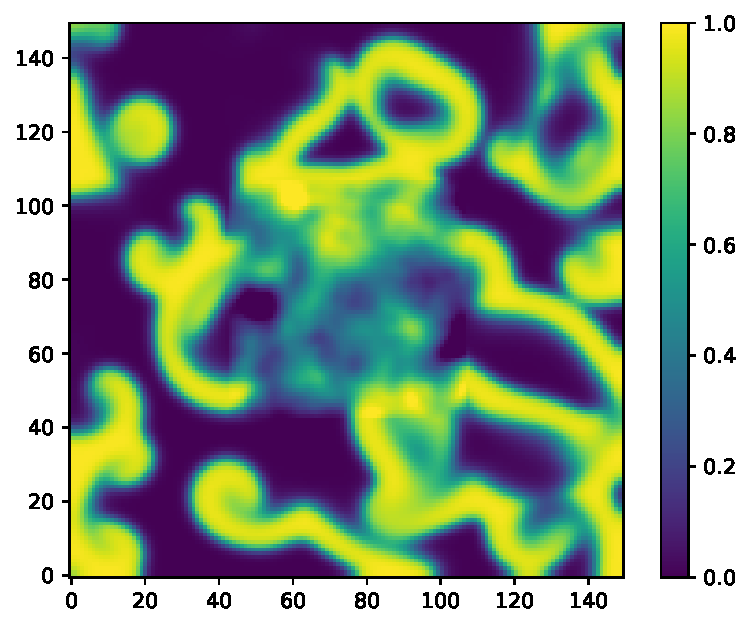
\includegraphics[height=2.5in]{figures/results/inner_cross_prediction/barkley_u_inner_esn_low_penalty.pdf}
		\setcapmargin[1cm]{0.5cm}
  		\caption{Vorhersage des \textsc{ESN}s mit $\lambda=0.05$}
	\end{subfigure}
	\caption{Graphische Darstellung der $u$-Variable des \textit{Barkley}-Modells für den $1000$. Zeitschritt des Evaluationsdatensatzes. Links ist die Vorhersage des \textsc{ESN}s mit starker und rechts mit schwacher Regularisierung dargestellt.}
	\label{fig:exp_inner_cross_barkley_esn_comparison}
\end{figure} 



Um den Einfluss der Regularisierung hervorzuheben, sind in Abbildung \ref{fig:exp_inner_cross_barkley_esn_comparison} die Vorhersagen des optimalen Reservoirs mit der hohen Regularisierung ($\lambda=\num{5e4}$) und eines zuvor ermittelten Reservoirs mit einer geringeren Regularisierung ($\lambda=0.05$) exemplarisch für das \textit{Barkley}-Modell dargestellt.
Im Falle der starken Regularisierung ist die Vorhersage stark verschwommen und so wird beinahe der Mittelwert der Erregung anstelle der feineren Strukturen vorhergesagt. Dagegen wird bei der geringeren Regularisierung eine feinere Struktur bestimmt. \improvement{Add details?}
Zudem ist in Abbildung \ref{fig:exp_inner_cross_barkley_esn_error_dependency_comparison} die Abhängigkeit des mittleren quadratischen Fehlers für jene beiden Reservoirs dargestellt. Dabei ist zu erkennen, dass für geringe Abstände die Vorhersage mit der kleinen Regularisierung deutlich kleinere Fehler verursacht, wohingegen ab einem Abstand von fünf Gitterpunkten eine stärkere Regularisierung geringere Fehler erzeugt. Des Weiteren scheint der Fehler dabei schnell gegen eine obere Schranke zu konvergieren. Dies lässt sich damit vereinbaren, dass dieses Reservoir hauptsächlich noch den Mittelwert der Dynamik vorhersagt.

\begin{figure}[h]
	\centering
	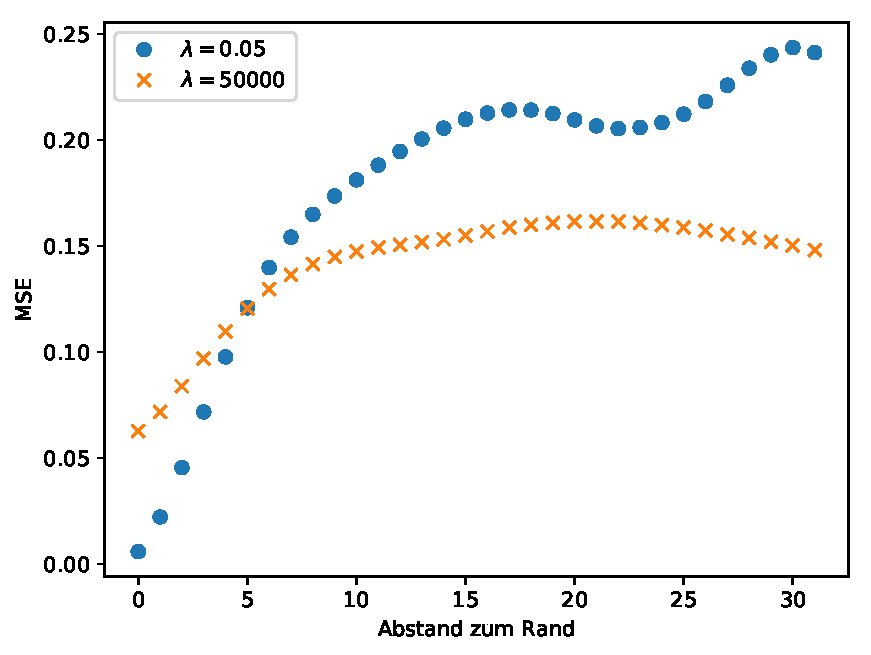
\includegraphics[height=3.5in]{figures/results/inner_cross_prediction/inner_errors.pdf}
	\setcapmargin[1cm]{0.5cm}
	\caption{Graphische Darstellung der Abhängigkeit des MSE für die Vorhersage der $u$-Variable des \textit{Barkley}-Modells vom Abstand zum Rand des vorherzusagenden Gebiets. In Blau ist die Abhängigkeit für das \textsc{ESN}s mit starker und in Orange für das mit schwacher Regularisierung dargestellt.}
	\label{fig:exp_inner_cross_barkley_esn_error_dependency_comparison}
\end{figure} 


\FloatBarrier
\subsection{Vergleich}
Zuerst kann bemerkt werden, dass für den \textsc{NN}- und den \textsc{RBF}-Ansatz der optimale Wert für die Randdicke $b=1$ lautet, wohingegen bei den \textsc{ESN}s Werte mit $b > 1$ besserer Ergebnisse liefern. Dieser Unterschied lässt sich dadurch erklären, dass das Eingangssignal für das \textsc{ESN} nicht vollständig genutzt worden ist, sondern durch die Verwendung der dünnbesetzten Eingangsmatrix $\mathbf{W_{in}}$ nur einzelne zufällig ausgewählte Punkte genutzt worden sind. Somit können in diesem Fall, durch einen breiteren Rand, Eingangssignale aus einer größeren Menge an unterschiedlichen Signalen gewählt werden.
\improvement{Make this more clear.}
Für einen genaueren Vergleich der drei Methoden bietet es sich an die Ergebnisse für den größten $a$-Wert durchzuführen, der mit allen drei Ansätzen betrachtet worden ist. Dieser Anforderung entspricht der Wert $a=64$. Eine Übersicht der verschiedenen Ergebnisse ist in Tabelle \ref{tab:exp_inner_cross_comparison_results} zu finden.

\begin{table}[H]
	\centering
	\captionsetup{width=0.9\linewidth}
	\begin{tabular}{cccccccc}
		\hline
		\multicolumn{1}{c}{} & \multicolumn{3}{c}{Barkley} & \multicolumn{3}{c}{Mitchell-Schaeffer}		\\
		%\cline{2-7}
		\multicolumn{1}{c}{} & NN & RBF & ESN & NN & RBF & ESN \\
		
		\hline
		
		Laufzeit [s] 	& 14754		&  	1845	& \textbf{1206}		&	20272 	& 1756		& \textbf{1089}		 \\
		MSE 			& 0.24599	& 0.13615 	& \textbf{0.12882}	&	0.09283	& 0.05588	& 	\textbf{0.05464}  \\
		NRMSE 			& 1.2963	& 0.9805 	& \textbf{0.9438}	&	1.1837	& 1.0094	& \textbf{0.9081} 	 \\
		\hline 
	\end{tabular} 
	\caption{Vergleich der benötigten Laufzeit und des erreichten Fehlers der drei Ansätze für das \textit{Mitchell-Schaeffer}- und das \textit{Barkley}-Modell für $a=64$, welche zu den geringsten Fehlern führen.}
	\label{tab:exp_inner_cross_comparison_results}
\end{table}

Ergänzend ist ein grafischer Vergleich der normalisierten Fehlerwerte NRMSE für alle untersuchen Abmessungen $a$ durchgeführt worden, welcher in Abbildung \ref{fig:inner_prediction_error_size_comparison_barkley} für das \textit{Barkley}-Modell zu finden ist. Eine analoge Darstellung für das \textit{Mitchell-Schaeffer}-Modell ist in Abbildung \ref{fig:apx_inner_prediction_error_size_comparison_ms} aufgetragen. Wieder zeigt sich, dass die Vorhersagen der klassischen Methoden einen höheren Fehler haben. Während der \textsc{NN}-Ansatz bei beiden Modellen schlechtere Ergebnisse als die Vorhersage mittels des Mittelwertes liefert, sind die radialen Basisfunktionen und die \textsc{ESN}s geringfügig besser als diese für $a=64$. Dabei erreichen die \textsc{ESN}s und radialen Basisfunktionen in etwa die gleiche Genauigkeit. Da der NRMSE für beide Methoden nah an $1.0$ liegt, ist die Vorhersage kaum besser als die Vorhersage mittels des Mittelwertes. Die Vorhersagequalität reicht bei keiner der drei Methoden aus, um sie tatsächlich sinnvoll verwenden zu können.

\begin{figure}[H]
	\centering
	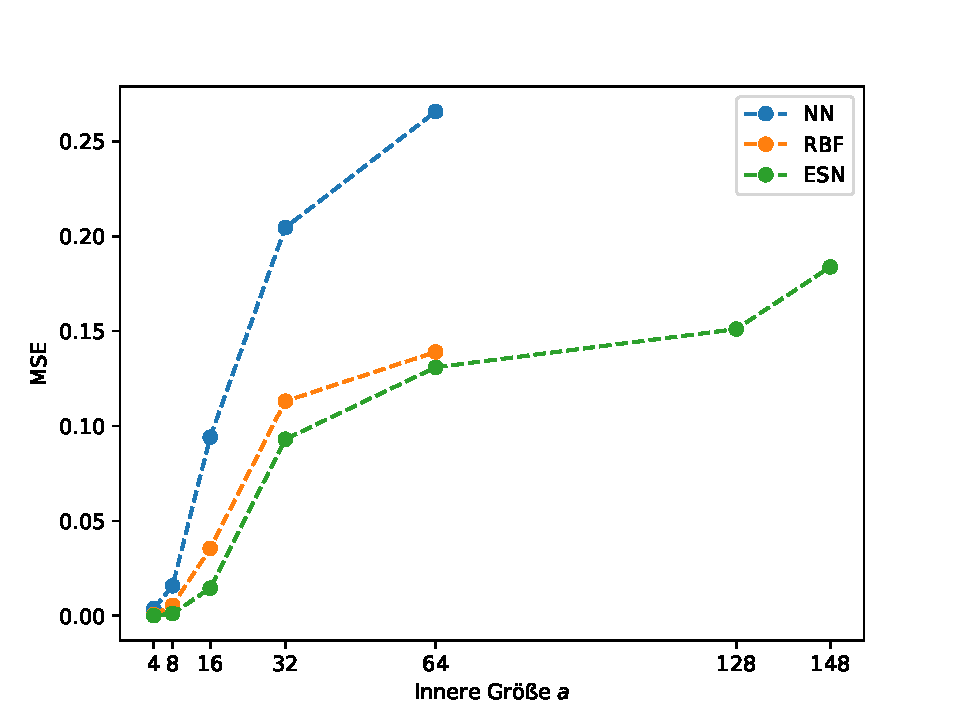
\includegraphics[height=3.7in]{figures/results/inner_cross_prediction/barkley_error_size_comparison.pdf}
	\caption{Darstellung des normalisierten Fehlerwertes NRMSE für die drei Ansätze in Abhängigkeit von der Größe $a$ des vorherzusagenden Bereichs für das \textit{Barkley}-Modell.}
	\label{fig:inner_prediction_error_size_comparison_barkley}
\end{figure}
 


Des Weiteren wächst der Fehler mit steigender Größe des vorherzusagenden Bereiches bei allen drei Ansätzen an. Es ist somit zu vermuten, dass dies nicht nur eine reine Beschränkung der einzelnen Methoden ist, sondern dass es womöglich eine Eigenschaft der betrachteten Modelle ist. \\
\improvement{Add comparison images} 

In Abbildung \ref{fig:exp_inner_cross_barkley_result} werden exemplarisch die aus den drei Ansätzen resultierenden Felder der Spannungsvariable $u(t)$ des \textit{Barkley}-Modells, zusammen mit dem originalen Feld, dargestellt. Eine analoge Darstellung für das \textit{Mitchell-Schaeffer}-Modell ist im Anhang als Abbildung \ref{fig:apx_inner_cross_mitchell_result} zu finden. Es fällt auf, dass sowohl die Vorhersage der \textsc{RBF} als auch die des \textsc{ESN} stark verschwommen ist und kaum Details zeigt. Im Gegensatz dazu macht der \textsc{NN}-Ansatz eine sehr scharfe Vorhersage. Dies ist dahingehend interessant, als das zum einen jeder Bildpunkt einzeln vorhersagt wird, und zum anderen immer die nächsten fünf Nachbarn im Zustandsraum genutzt werden. 

\begin{figure}[H]
	\centering
	\begin{subfigure}{.5\textwidth}
		\centering
		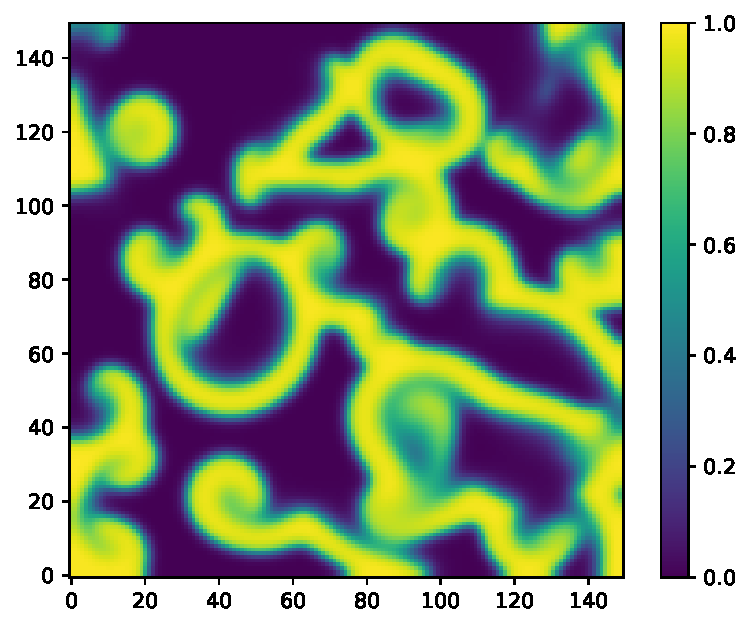
\includegraphics[height=2.5in]{figures/results/inner_cross_prediction/barkley_u_inner_original.pdf}
		\setcapmargin[1cm]{0.5cm}
		\caption{Echte Erregung des Modells}
		\label{fig:exp_inner_cross_barkley_result_orig}
	\end{subfigure}%
	\begin{subfigure}{.5\textwidth}
		\centering
		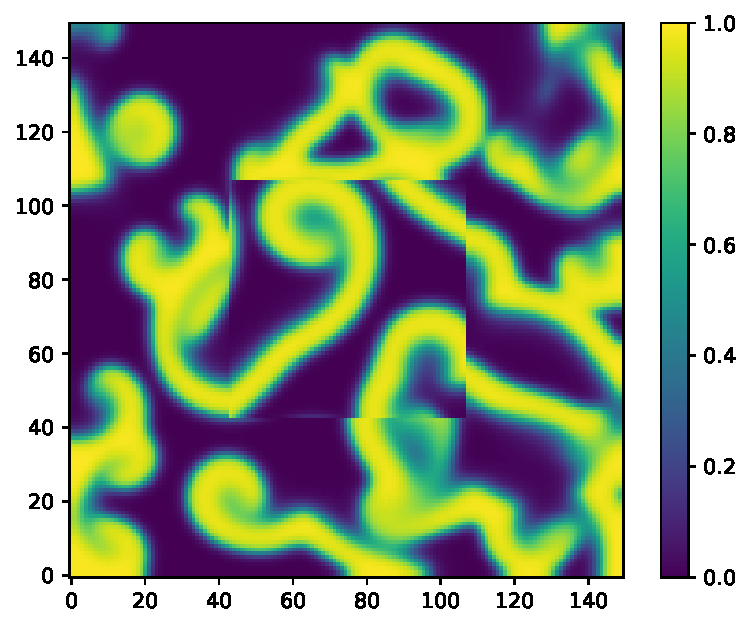
\includegraphics[height=2.5in]{figures/results/inner_cross_prediction/barkley_u_inner_nn.pdf}
		\setcapmargin[1cm]{0.5cm}
  		\caption{Vorhersage des \textsc{NN}-Ansatzes}
  		\label{fig:exp_inner_cross_barkley_result_nn_pred}
	\end{subfigure}
	\begin{subfigure}{.5\textwidth}
		\centering
		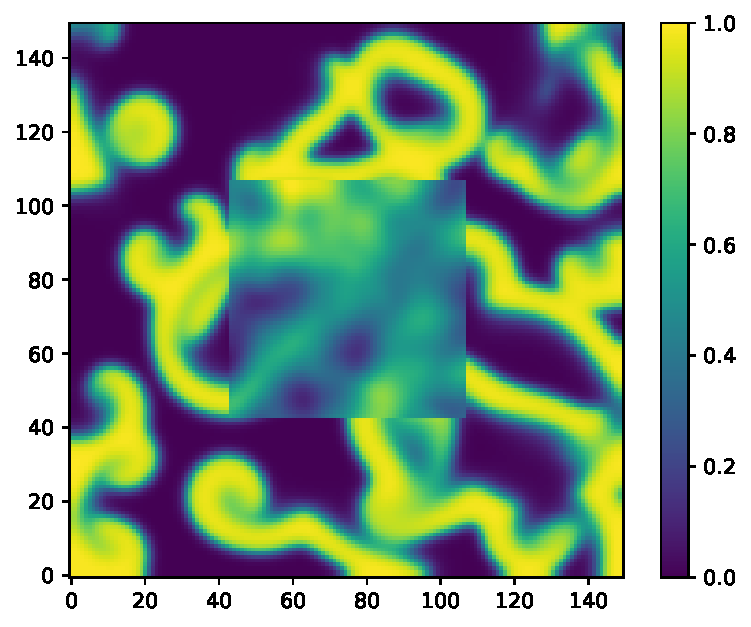
\includegraphics[height=2.5in]{figures/results/inner_cross_prediction/barkley_u_inner_rbf.pdf}
		\setcapmargin[1cm]{0.5cm}
  		\caption{Vorhersage des \textsc{RBF}-Ansatzes}
  		\label{fig:exp_inner_cross_barkley_result_rbf_pred}
	\end{subfigure}%
	\begin{subfigure}{.5\textwidth}
		\centering
		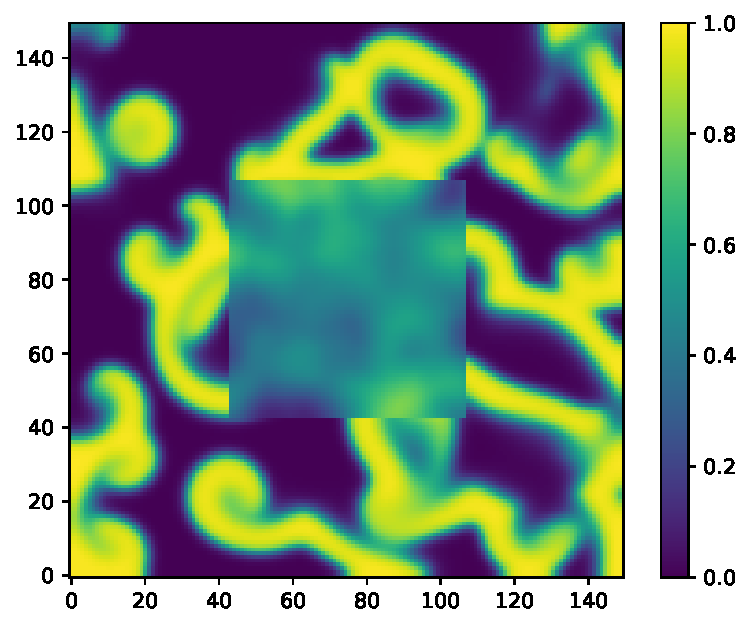
\includegraphics[height=2.5in]{figures/results/inner_cross_prediction/barkley_u_inner_esn.pdf}
		\setcapmargin[1cm]{0.5cm}
  		\caption{Vorhersage des \textsc{ESN}}
  		\label{fig:exp_inner_cross_barkley_result_esn_pred}
	\end{subfigure}
	\caption{Graphische Darstellung der $u$-Variable des \textit{Barkley}-Modells für den $1000$. Zeitschritt des Evaluationsdatensatzes für $a=64$. Oben links ist das tatsächliche Feld des Modells zu sehen. Danach folgenden im Uhrzeigersinn die Vorhersagen des \textsc{NN}-Ansatzes, des \textsc{RBF}-Ansatzes und des \textsc{ESN}.}
	\label{fig:exp_inner_cross_barkley_result}
\end{figure} 

Daraus können zwei Konsequenzen folgen. Erstens spricht die hohe Auflösung dafür, dass die Vorhersage nahezu perfekt einem Bereich aus den Trainingsdaten entspricht. Da die Vorhersage aber (zumindest in diesem Moment) nicht gut mit dem Original übereinstimmt, bedeutet dies, dass die Verzögerungskoordinaten, die genutzt worden sind, den Bereich nicht eindeutig beschreiben. Zweitens kann daraus auch gefolgert werden, dass für diese Aufgabe die Länge der Trainingsdaten zu gering gewählt worden ist. 
